%-*- coding: utf-8 -*-
\documentclass[11pt,a4paper,french,twoside,openright]{article}
\usepackage[utf8]{inputenc}
\usepackage[T1]{fontenc}
\usepackage{graphicx}%pour insérer images et pdf entre autres
	\graphicspath{{images/}}%pour spécifier le chemin d'accès aux images
\usepackage[left=2.5cm,right=2.5cm,top=2.5cm,bottom=2.5cm]{geometry}%réglages des marges du document selon vos préférences ou celles de votre établissemant
\usepackage[Lenny]{fncychap}%pour de jolis titres de chapitres voir la doc pour d'autres styles.
\usepackage{babel}
\usepackage[babel=true]{csquotes} % csquotes va utiliser la langue définie dans babel
\usepackage{LastPage}

\usepackage{fancyhdr}%pour les entêtes et pieds de pages
	\setlength{\headheight}{14.2pt}% hauteur de l'entête
        \chead{\textbf{VITAMEAL}}
        \lhead{}
        \rhead{}
	\cfoot{Formation Ingénieur Informatique en alternance - Première année}
	\lfoot{\textbf{CNAM}}%
  	\rfoot{\textbf{\thepage/\pageref{LastPage}}}
 	\renewcommand{\headrulewidth}{0.4pt}%trait horizontal pour l'entête
  	\renewcommand{\footrulewidth}{0.4pt}%trait horizontal pour les pieds de pages

\usepackage[french]{nomencl}
\makenomenclature
\usepackage{hyperref}
\usepackage{mathtools}
\begin{document}
\pagestyle{fancy}

\begin{center}\bfseries\Huge
COMPTE RENDU DE TÉLÉCONFÉRENCE
\end{center}

\textbf{Du      :} mercredi 28/06/2017 à 20h30

\textbf{Objet   :} Avancement projet VITAMEAL

\textbf{Présents:} Nicolas SYMPHORIEN, Jean-Félix BENITEZ

\textbf{Absente :} Sonia OTHMANI (excusée).

\textbf{Diffusion:} Nicolas SYMPHORIEN, Sonia OTHMANI, Jean-Félix BENITEZ

\hrulefill

\section{Conception}
Avancement du travail de Nicolas:
\begin{itemize}
\item Intégration des classes du domaines misent en oeuvre dans les cas d'utilisations.
\item 2 maquettes IHM faites.
\item Conception dynamique (diagramme de séquences) en cours
\item Conception statique (diagramme des classes) et codage en cours.
\item \textbf{Problème} (non bloquant) avec hibernate qui crée des tables déjà existantes (code sous \emph{GitHub}).
\end{itemize}

Avancement du travail Jean-Félix:
\begin{itemize}
\item Diagramme de séquences détaillé, fait.
\item Diagramme des classes de l'élaboration des menus en cours, voir \autoref{ClassesElaborationMenu}
\item Description écrite de l'algorithme d'élaboration des menus à finaliser.
\end{itemize}

Nous continuons à travailler sur la conception et le codage durant la semaine, de manière à pouvoir consacrer le début du week-end à la préparation des cours de la semaine prochaine (BDD plus Anglais, notament). \textbf{Nous remonterons sous GitHub dimanche matin au plus tard, nos travaux de conceptions avec leurs descriptions, afin de pouvoir travailler le rapport et la présentation dimanche après-midi.}

\section{Prochain rendez-vous}
\textbf{dimanche 02/07/2017 20h30}

\begin{figure}
  \centering
      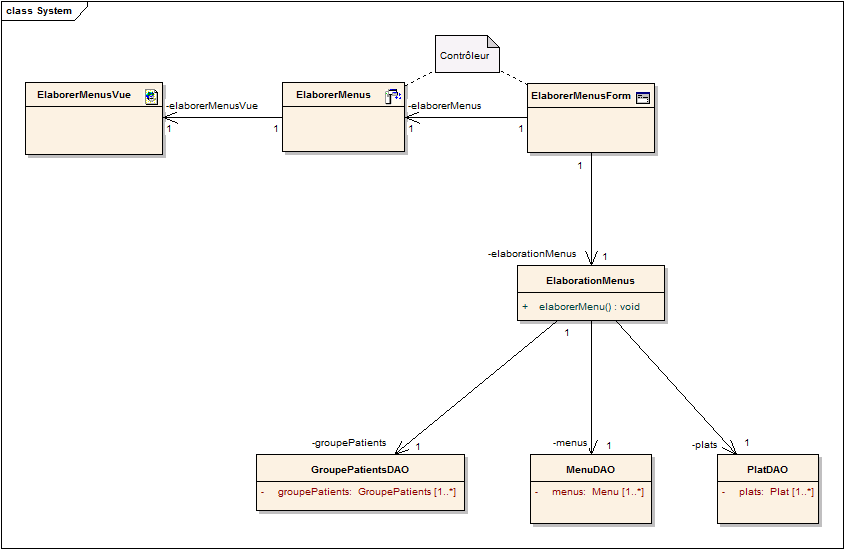
\includegraphics[width=1.00\textwidth]{../../CasDUtilisations/MenuGen/Classes/EMC.png} %
\caption{Classes Élaboration Menus}
\label{ClassesElaborationMenu}
\end{figure}

\end{document}
